\section{Discussão geral}

\label{sec:discussao}

\subsection{Interdependência dos fenômenos de microssegregação e reação bainítica}

Os resultados experimentais do presente trabalho mostram que a ocorrência de reações competitivas é inevitável durante a aplicação do processo de têmpera e partição à presente liga de ferro fundido nodular. Em particular, a cinética global da reação bainítica é acelerada pela presença de martensita. No entanto, a rejeição de carbono durante o crescimento da ferrita bainítica, isenta de carbonetos, auxilia no enriquecimento em carbono da austenita.

Embora a formação de ferrita bainítica beneficie a estabilização da austenita no ferro fundido, aços modernos planejados para serem submetidas ao processo T\&P levam adições de elementos de liga que aumentam a temperabilidade e, portanto, atrasam a reação bainítica \cite{Santofimia2011a,DeKnijf2015}. A reação bainítica consome a austenita, diminuindo assim as quantidades finais de austenita estabilizada. Por sua vez, a ocorrência da reação bainítica pode ser entendida com base na temperatura Bs, acima da qual a reação bainítica não ocorre. Algumas equações empíricas para o cálculo da temperatura Bs são disponíveis na literatura, tal como a equação proposta por \citaremsentenca{VanBohemen2012}:

\begin{align}
  \text{Bs (\SI{}{\degreeCelsius})} &= 839 - 86 \%w_{Mn}^\gamma - 23 \%w_{Si}^\gamma - 67 \%w_{Cr}^\gamma - 33 \%w_{Ni}^\gamma \nonumber \\
  & - 75 \%w_{Mo}^\gamma - 270 \left[ 1 - \exp\left( -\SI{1.33}{} \%w_C^\gamma \right) \right]
  \label{eq:Bs}
\end{align}

Caso a etapa de partição seja conduzida acima da temperatura Bs, a reação bainítica não ocorrerá. Note-se que na equação \ref{eq:Bs} o manganês é o elemento cujo efeito na temperatura Bs é mais pronunciado, uma vez que o termo $\%w_{Mn}^\gamma$ é acompanhado do coeficiente de maior magnitude. Devido a este efeito, ligas modernas fazem uso de adições significativas de Mn. Na Tabela \ref{tab:comp_literatura_Bs} são mostradas as composições de algumas ligas exploradas na literatura para o tratamento T\&P e as respectivas temperaturas Bs calculadas pela equação \ref{eq:Bs}.

\begin{table}
  \caption{Temperaturas Bs calculadas para diferentes ligas em que se foi aplicado o processo T\&P.}
  \begin{tabular}{c c c}
  \thickhline
  Referência & Composição da austenita & Bs (\SI{}{\degreeCelsius}) \\
  \hline
  \citaremsentenca{Santofimia2011a} & Fe--0,204C--2,5Mn--1,47Ni--1,01Cr--1,5Si & 409,2\\
  \citaremsentenca{Hajyakbary2016} & Fe--0,3C--1,6Si--3,5Mn & 412,4\\
  \citaremsentenca{Toji2015} & Fe--1,07C--2,2Si--2,9Mn & 334,1\\
  \citaremsentenca{Toji2015} & Fe--0,59C--2Si--2,9Mn & 396,8\\
  Presente trabalho & Fe--0,76C--0,21Mn--2,5Si & 591,7\\
  \thickhline
  \end{tabular}
  \label{tab:comp_literatura_Bs}
\end{table}

Nota-se que as ligas apresentadas na Tabela \ref{tab:comp_literatura_Bs} apresentam teores de Mn mais elevados e, portanto, Bs significativamente menores do que o ferro fundido estudado neste trabalho, em que a Bs é igual \SI{591.7}{\degreeCelsius}. A realização da etapa de partição a temperaturas superiores a \SI{591.7}{\degreeCelsius} na presente liga é inviável, uma vez que nessas temperaturas o material é passível de precipitar cementita a partir da martensita, o que inviabilizaria a partição de carbono. Por outro lado, o aumento em 2\% em peso no teor de Mn no ferro fundido abaixaria a temperatura Bs para aproximadamente \SI{400}{\degreeCelsius}, na qual o tratamento de partição seria possível sem a ocorrência de precipitação de cementita e reação bainítica. No entanto, ligas elevadas adições de manganês e outros elementos de liga tendem a possuir os efeitos de microssegregação aumentados. 

Ao contrário de produtos siderúrgicos, que são submetidos a etapas de deformação (e.g., laminação, forjamento) e tratamentos de homogeneização, que contribuem para a diminuição da segregação inerente da etapa de lingotamento, ferros fundidos não são submetidos a tais processos. Ainda que fosse tecnologicamente viável aplicar etapas de deformação e tratamentos de homogeneização a ferros fundidos nodulares, tais etapas impediriam fazer uso de uma das principais vantagens da produção de peças fundidas, a produção de peças próximas da forma final (\enfase{near net shape}). Dessa forma, a microssegregação inerente ao processo de solidificação, embora indesejada, é uma variável que sempre deve ser considerada. 

Um dos efeitos da microssegregação na evolução microestrutural durante o tratamento T\&P é a heterogeneidade na distribuição da martensita formada na etapa de têmpera. Contornos de célula eutética apresentam menores frações de martensita, enquanto regiões próximas a nódulos de grafita apresentam maiores frações transformadas. Isto tem como principais efeitos diminuir a quantidade local de carbono (na forma de martensita) disponível para partição de carbono para a austenita e alterar a cinética local da reação bainítica. Na ausência de martensita, a reação bainítica torna-se mais lenta e a estabilização da austenita nestas regiões tende a demorar mais para acontecer. Os resultados de EBSD mostram que para tempos curtos de partição a estabilização da austenita ocorre nas regiões de maior fração de martensita, enquanto que regiões de contornos de célula apresentam grandes quantidades de martensita fresca, detrimental para as propriedades mecânicas do material. Assim, tempos de partição mais longos são necessários para que toda a austenita retida seja estabilizada no material. Caso a martensita fosse mais homogeneamente distribuída no material, tempos menores de partição seriam suficientes para que a austenita fosse estabilizada. Isto é conseguido abaixando a temperatura de têmpera, mas isto tem como efeito prejudicial a diminuição das quantidades finais de austenita retida.

Em suma, os efeitos de microssegregação e reação bainítica estão relacionados um ao outro. Adições de elementos de liga tendem a diminuir a temperatura Bs, mas ao mesmo tempo levam ao aumento da microssegregação. Por sua vez, a microssegregação leva a uma distribuição heterogênea de martensita ao longo do material, que causa a cinética da reação bainítica ser diferente em diferentes regiões do material. 



\subsection{Efeito da precipitação de carbonetos na martensita na partição de carbono}

A precipitação de carbonetos na martensita foi observada diretamente pela caracterização metalográfica das amostras temperadas e particionadas. A cinética de precipitação dos carbonetos é rápida, de modo que carbonetos foram observados mesmo nas amostras particionadas nos menores tempos (0 e 30~s). Não foram observados carbonetos na amostra temperada a \SI{170}{\degreeCelsius}, mantida nesta temperatura por 1~min e resfriada até a temperatura ambiente. Isto evidencia que a formação dos carbonetos acontece durante a etapa de aquecimento desde a temperatura de têmpera até a temperatura de partição.

Análises de difração de raios X com radiação síncrotron possibilitaram identificar os carbonetos formados após partição a \SI{450}{\degreeCelsius} como sendo cementita. Para as menores temperaturas de 300 e \SI{375}{\degreeCelsius} os carbonetos foram identificados como sendo de transição do tipo $\eta$, de estrutura ortorrômbica. A precipitação de carbonetos de transição a baixas temperaturas e cementita a altas temperaturas foi corroborada por um experimento crítico de dilatometria, em que uma amostra temperada foi revenida por aquecimento contínuo até \SI{700}{\degreeCelsius} a uma taxa de \SI{12}{\degreeCelsius/s}. As curvas de dilatometria deste teste apresentaram contrações características das reações de precipitação de carbonetos de transição e de cementita durante o revenimento da martensita a 120 e \SI{430}{\degreeCelsius}, respectivamente.

Apesar da presença de carbonetos na martensita, resultados de EBSD revelaram uma evidência indireta da partição de carbono desde a mistura de martensita + carbonetos ($\alpha' + \theta$) para a austenita ($\gamma$) em uma amostra particionada a \SI{375}{\degreeCelsius} por 30~s. Nesta condição, filmes de austenita retida próximos a placas de martensita foram observadas nos mapas de fases obtidos por EBSD. Assume-se que estes filmes foram estabilizados pelo enriquecimento em carbono da austenita. Como não há placas de ferrita bainítica próximas a estas regiões, que também poderiam explicar o enriquecimento em carbono desta austenita, conclui-se que estes filmes de austenita foram enriquecidos pela partição de carbono da mistura de martensita + carbonetos para a austenita.

A partição de carbono da martensita para a austenita, mesmo com a presença de carbonetos, é justificada pelo modelo ERC$\theta$ proposto por \citaremsentenca{Toji2015}. A força motriz para partição de carbono é a diferença de potenciais químicos do carbono $\mu_C$ entre uma fase e outra. A precipitação de carbonetos na martensita diminui a diferença de $\mu_C$ entre a $\alpha' + \theta$ e $\gamma$ ($\mu_C^{\alpha' + \theta}$ e $\mu_C^\gamma$, respectivamente), mas, desde que $\mu_C^{\alpha' + \theta} > \mu_C^\gamma$, a partição de carbono ainda é termodinamicamente possível. Caso contrário, o carbono difundiria de $\gamma$ para $\alpha' + \theta$. Quanto menor é a energia livre do carboneto precipitado na martensita (quanto mais estável é o carboneto), menor é a diferença entre $\mu_C^{\alpha' + \theta}$ e $\mu_C^\gamma$ e mais difícil se torna a partição de carbono para a austenita. 

Neste trabalho, o teor de carbono na austenita calculado assumindo o modelo ERC$\theta$ com a precipitação de ortocementita a \SI{375}{\degreeCelsius} é menor (0,277\%) do que a composição inicial da liga (0,76\%). Isto significa que quando a precipitação de ortocementita acontece na martensita, a partição de carbono para a austenita é impossível. Em relação aos carbonetos de transição, embora não existam dados termodinâmicos disponíveis sobre estas fases, é seguro afirmar que estes carbonetos são mais energéticos (menos estáveis) do que a ortocementita. Carbonetos de transição toleram grandes quantidades de silício em solução sólida, enquanto que a ortocementita possui solubilidade em silício virtualmente igual a zero. Na cementita, o parâmetro de interação Si-C é negativo, o que significa que na cementita a formação de pares atômicos Si-Si e C-C é mais energeticamente favorável do que pares Si-C, o que explica a baixa solubilidade em Si da cementita. Não há motivos para acreditar que nos carbonetos de transição o parâmetro de interação Si-C seja significativamente diferente daquele na cementita. Como consequência, o alto teor de Si observado nos carbonetos de transição é refletido em uma maior energia livre em relação à da cementita. Dessa forma, é razoável esperar que a precipitação de carbonetos de transição na martensita não cause uma diminuição significativa de $\mu_C^{\alpha' + \theta}$ e a partição de carbono de $\alpha' + \theta$ para $\gamma$ ainda seja termodinamicamente possível. 

Com efeito, trabalhos na literatura tem demonstrado que a precipitação de carbonetos de transição na martensita durante o processo T\&P não é impedimento para a partição de carbono \cite{Seo2016,Hajyakbary2016}. Por exemplo, \citaremsentenca{Hajyakbary2016} observaram a precipitação de carbonetos $\epsilon$ de auto-revenimento durante a etapa de têmpera do tratamento T\&P. Durante a etapa de partição estes carbonetos foram redissolvidos, evidenciando que a partição de carbono de $\alpha' + \theta$ para $\gamma$ acontece mesmo na presença de carbonetos $\epsilon$.

Assim, a evidência de partição de carbono de $\alpha' + \theta$ para $\gamma$ a \SI{375}{\degreeCelsius} é justificada pelo fato de que os carbonetos de transição $\eta$ não causam um abaixamento significativo do potencial químico de carbono $\mu_C^{\alpha' + \theta}$. De forma semelhante, a \SI{300}{\degreeCelsius}, em que também é a observada a precipitação de carbonetos $\eta$, a partição de carbono também é termodinamicamente possível. Por outro lado, a \SI{450}{\degreeCelsius}, em que é observada a precipitação de cementita, a partição de carbono é desfavorecida, já que a cementita causa uma maior diminuição de $\mu_C^{\alpha' + \theta}$.



\subsection{Interação entre reação bainítica e precipitação de carbonetos na redistribuição de carbono}

Embora para tempos curtos haja evidência de partição de carbono de $\alpha' + \theta$ para $\gamma$, para longos tempos de partição não foram observadas mudanças apreciáveis na fração dos carbonetos. A análise de carbono por EPMA sobre uma placa de martensita com carbonetos em uma amostra particionada a \SI{375}{\degreeCelsius} por 15~min mostra que o teor médio de carbono em $\alpha' + \theta$ ($\overline{c^{\alpha' + \theta}}$) é maior (0,85\%) do que a composição inicial da austenita (0,76\%).

Este comportamento pode ser explicado de acordo como o carbono particionado de $\alpha' + \theta$ para $\gamma$ interage com o carbono rejeitado para $\gamma$ durante o crescimento da ferrita bainítica $\alpha_b$. No modelo cinético desenvolvido neste trabalho, diferentes considerações termodinâmicas são assumidas para as interfaces $\alpha' + \theta/\gamma$ e $\alpha_b/\gamma$. Nas interfaces $\alpha_b/\gamma$ o limite WBs se aplica; nas interfaces $\alpha' + \theta/\gamma$ é assumido que as condições do modelo ERC$\theta$ se aplicam. A composição interfacial da austenita $c^\gamma_{int}$ calculada pelo modelo ERC$\theta$ varia de acordo com a energia livre dos carbonetos precipitados. Assim, diferentes cenários são observados dependendo do valor de $c^\gamma_{int}$ estabelecido para diferentes valores do potencial químico $\mu_C^{\alpha' + \theta}$. As simulações mostram que quando $c^\gamma_{int}$ é maior do que a composição inicial da austenita e menor do que a composição WBs, $\alpha' + \theta$ inicialmente tem seu carbono particionado para $\gamma$. Para tempos longos, o carbono rejeitado para $\gamma$ pelo crescimento de $\alpha_b$ passa a interagir com o carbono particionado de $\alpha' + \theta$ para $\gamma$ e o carbono passa a fluir de $\gamma$ para $\alpha' + \theta$. Este comportamento é observado, por exemplo, quando $\mu_C^{\alpha' + \theta} = \SI{20}{kJ/mol}$ (ver Figura \ref{fig:discussao_particao}) e consegue explicar os resultados experimentais obtidos neste trabalho.
% Na Figura \ref{fig:discussao_particao} é mostrada a evolução do teor médio de carbono em $\alpha' + \theta$ ($\overline{c^{\alpha' + \theta}}$) em função do tempo de partição quando $\mu_C^{\alpha' + \theta} = \SI{20}{kJ}{mol}$. Fica claro que para tempos curtos $\overline{c^{\alpha' + \theta}}$ decresce até atingir um valor mínimo e para tempos longos $\overline{c^{\alpha' + \theta}}$ passa a aumentar.

\begin{figure}
  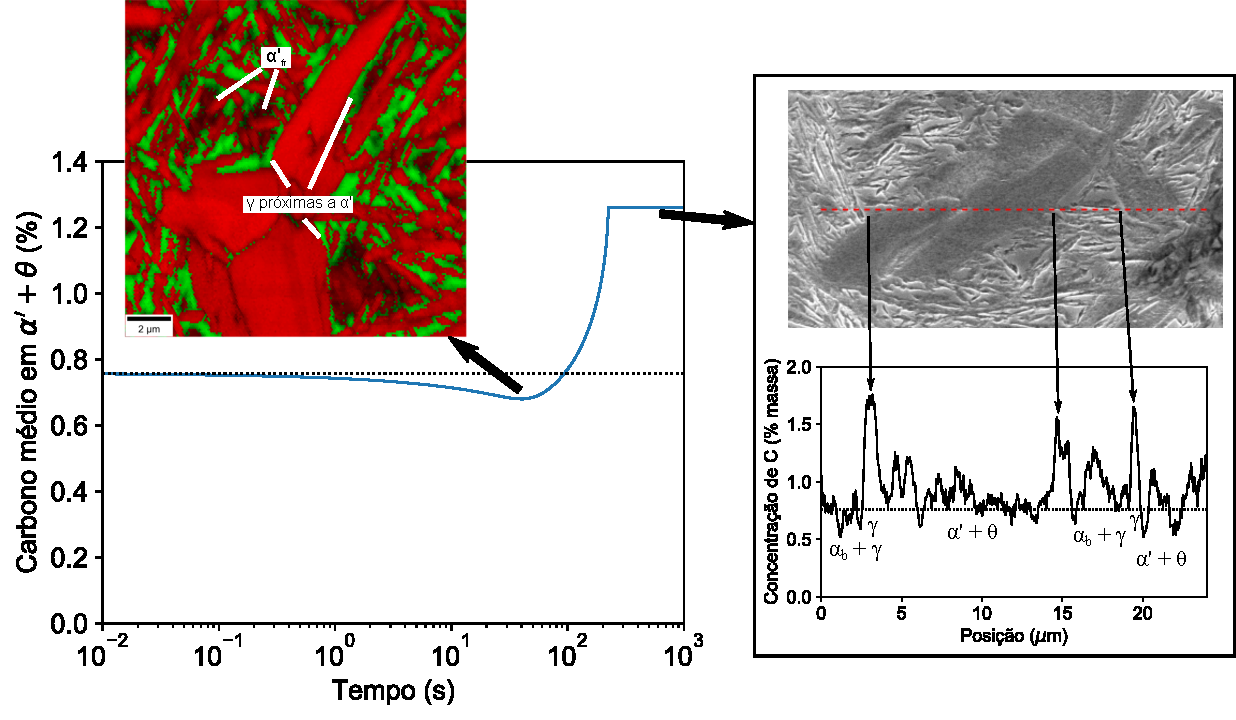
\includegraphics[width=\textwidth]{img/cpartition/coupled_cavg_mu20e3.pdf}
  \caption{Evolução do teor médio de carbono em $\alpha' + \theta$ ($\overline{c^{\alpha' + \theta}}$) calculado quando $\mu_C^{\alpha'+\theta} = \SI{20}{kJ/mol}$ mostrando que para tempos curtos $\overline{c^{\alpha' + \theta}}$ decresce, evidenciando a partição de carbono para $\gamma$, enquanto que para tempos longos $\overline{c^{\alpha' + \theta}}$ aumenta.}
  \label{fig:discussao_particao}
\end{figure}

Conclui-se que o carbono rejeitado durante a reação bainítica faz com que a partição de carbono de $\alpha' + \theta$ para $\gamma$ seja limitada aos primeiros instantes da etapa de partição. Dessa forma, a formação de ferrita bainítica é, efetivamente, o principal mecanismo de estabilização da austenita.

\subsection{Evolução microestrutural das amostras temperadas e particionadas}

Com base nas evidências experimentais e na discussão realizada nesta seção, a evolução microestrutural do ferro fundido nodular durante o tratamento de Têmpera e Partição pode ser sumarizada na seguinte sequência de etapas:

\begin{enumerate}
  \item Na etapa de austenitização a matriz do ferro fundido se transforma em austenita durante o aquecimento até a temperatura de austenitização. A temperatura de austenitização controla o teor de carbono médio na austenita e a fração de grafita. Temperaturas mais elevadas de austenitização levam a uma maior dissolução da grafita e uma austenita mais enriquecida em carbono. A microssegregação de solidificação tende a ser diminuída para tempos longos de austenitização. Para os parâmetros de austenitização utilizados no presente trabalho --- \SI{880}{\degreeCelsius} por 30~min --- a microssegregação persiste e seu efeito é observado na distribuição de martensita formada na etapa de têmpera. Devido à microssegregação, regiões de contornos de célula possuem maiores concentrações de carbono e manganês, enquanto regiões próximas aos nódulos de grafita apresentam maiores concentrações de silício e cobre.

  \item Na etapa de têmpera a austenita se transforma em martensita com morfologia de placas. A distribuição da martensita é heterogênea devido à microssegregação proveniente da etapa de solidificação do material. A temperatura Ms calculada para regiões de contorno de célula é menor do que em regiões próximas de nódulos de grafita. Consequentemente, regiões de contorno de célula apresentam menores frações de martensita, enquanto que próximo aos nódulos a fração é maior. A diminuição da temperatura de têmpera causa a homogeneização da distribuição da martensita e refina as regiões não transformadas de austenita. Assim, a diminuição da temperatura também causa o refino da produto bainítico formado na etapa de partição.
  % . Como o material é mantido na temperatura de têmpera por 1~min, a martensita sofre reações de revenimento, provavelmente a formação de agregados de carbono, conferindo a ela um aspecto diferenciado após ataque metalográfico. 

  \item Durante o aquecimento do material desde a temperatura de têmpera até a temperatura de partição ocorre a precipitação de carbonetos na martensita e o início da reação bainítica. O início da reação bainítica foi detectado por dilatometria a \SI{320}{\degreeCelsius} sob a taxa de aquecimento de \SI{10}{\degreeCelsius/s}. A reação bainítica nesta etapa poderia ser evitada utilizando uma taxa de aquecimento suficientemente elevada.

  \item Carbonetos são observados na martensita na fase inicial da etapa de partição. Para tempos curtos ocorre a partição de carbono de $\alpha' + \theta$ para $\gamma$. A reação bainítica também se inicia para tempos curtos de partição, acontecendo inicialmente sem a precipitação de carbonetos, com a formação de apenas ferrita bainítica. A ferrita bainítica, pobre em carbono, cresce expulsando carbono para a austenita, que passa a interagir com o carbono proveniente de $\alpha' + \theta$. A interação dos campos de difusão de carbono faz com que o carbono se difunda de $\gamma$ para $\alpha' + \theta$ para tempos longos de partição. Para tempos longos de partição é também observada a precipitação de carbonetos na bainita (segundo estágio da reação bainítica). Para \SI{450}{\degreeCelsius} esta etapa é rápida e faz com que a reação bainítica consuma toda a austenita após 15~min. Para 300 e \SI{375}{\degreeCelsius} a precipitação de carbonetos na bainita é lenta e, mesmo após 2~h, há quantidades significativas de austenita retida no material. Como discutido anteriormente, a cinética da reação bainítica é diferente para diferentes regiões do material, sendo mais rápida junto às regiões de nódulos de grafita, em que a reação é acelerada pela maior fração de martensita.

  \item Na etapa de resfriamento final a austenita não suficientemente estabilizada se transforma em martensita fresca. A martensita fresca se diferencia da martensita formada na etapa de têmpera por não ter sofrido reações de revenimento que diminuem o caráter frágil da martensita. A distribuição de martensita fresca é heterogênea ao longo do material, principalmente para tempos curtos de partição. Para tempos curtos, as regiões de contorno de célula, com pequena fração transformada de martensita, não tem tempo suficiente para se transformar em ferrita bainítica, que atua como mecanismo estabilizador da austenita retida. Dessa forma, a martensita fresca tende a se concentrar nestas regiões de contorno de célula.
\end{enumerate}

Quando os parâmetros de tratamento térmico são ajustados de modo a garantir que não haja nem martensita fresca e que quantidades apreciáveis de austenita retida sejam obtidas, a microestrutura final do ferro fundido temperado e particionado é multifásica, consistindo de martensita revenida, com precipitação de carbonetos, ferrita bainítica e austenita retida.

A caracterização das propriedades mecânicas da liga de ferro fundido temperada e particionada estudada neste trabalho foi feita por \citaremsentenca{Melado2018}, dentro do mesmo projeto em que se insere esta tese. \citaremsentenca{Melado2018} avaliou as propriedades mecânicas do material por ensaios de tração, tenacidade à fratura, ensaios de impacto e ensaios de fadiga. O estudo comparou as propriedades do ferro fundido temperado a 140 e \SI{170}{\degreeCelsius} e particionado a 300 e \SI{375}{\degreeCelsius} entre 15~min e 2~h com o ferro fundido austemperado (ADI) a 300 e \SI{375}{\degreeCelsius}. Os resultados de Melado mostraram que o ferro fundido T\&P apresenta alta resistência mecânica (limite de resistência à tração superior a \SI{1450}{MPa}) com valores consideráveis de ductilidade (até 9\%). O ferro fundido T\&P apresenta maior resistência em relação ao ADI, mas menores valores de ductilidade e energia absorvida no impacto. A elevada resistência provém da martensita revenida e do efeito de refino da microestrutura bainítica pela repartição da austenita não transformada. A Figura \ref{fig:banana_plot} mostra como as propriedades de resistência (limite de resistência à tração) e ductilidade do ferro fundido T\&P se relacionam com as propriedades de outras classes de ferros fundidos nodulares, mostrando que o material representa uma nova classe de ferros fundidos de alta resistência. Para a caracterização completa das propriedades mecânicas do ferro fundido T\&P, o leitor é referenciado à tese de Melado\cite{Melado2018}.

\begin{figure}
  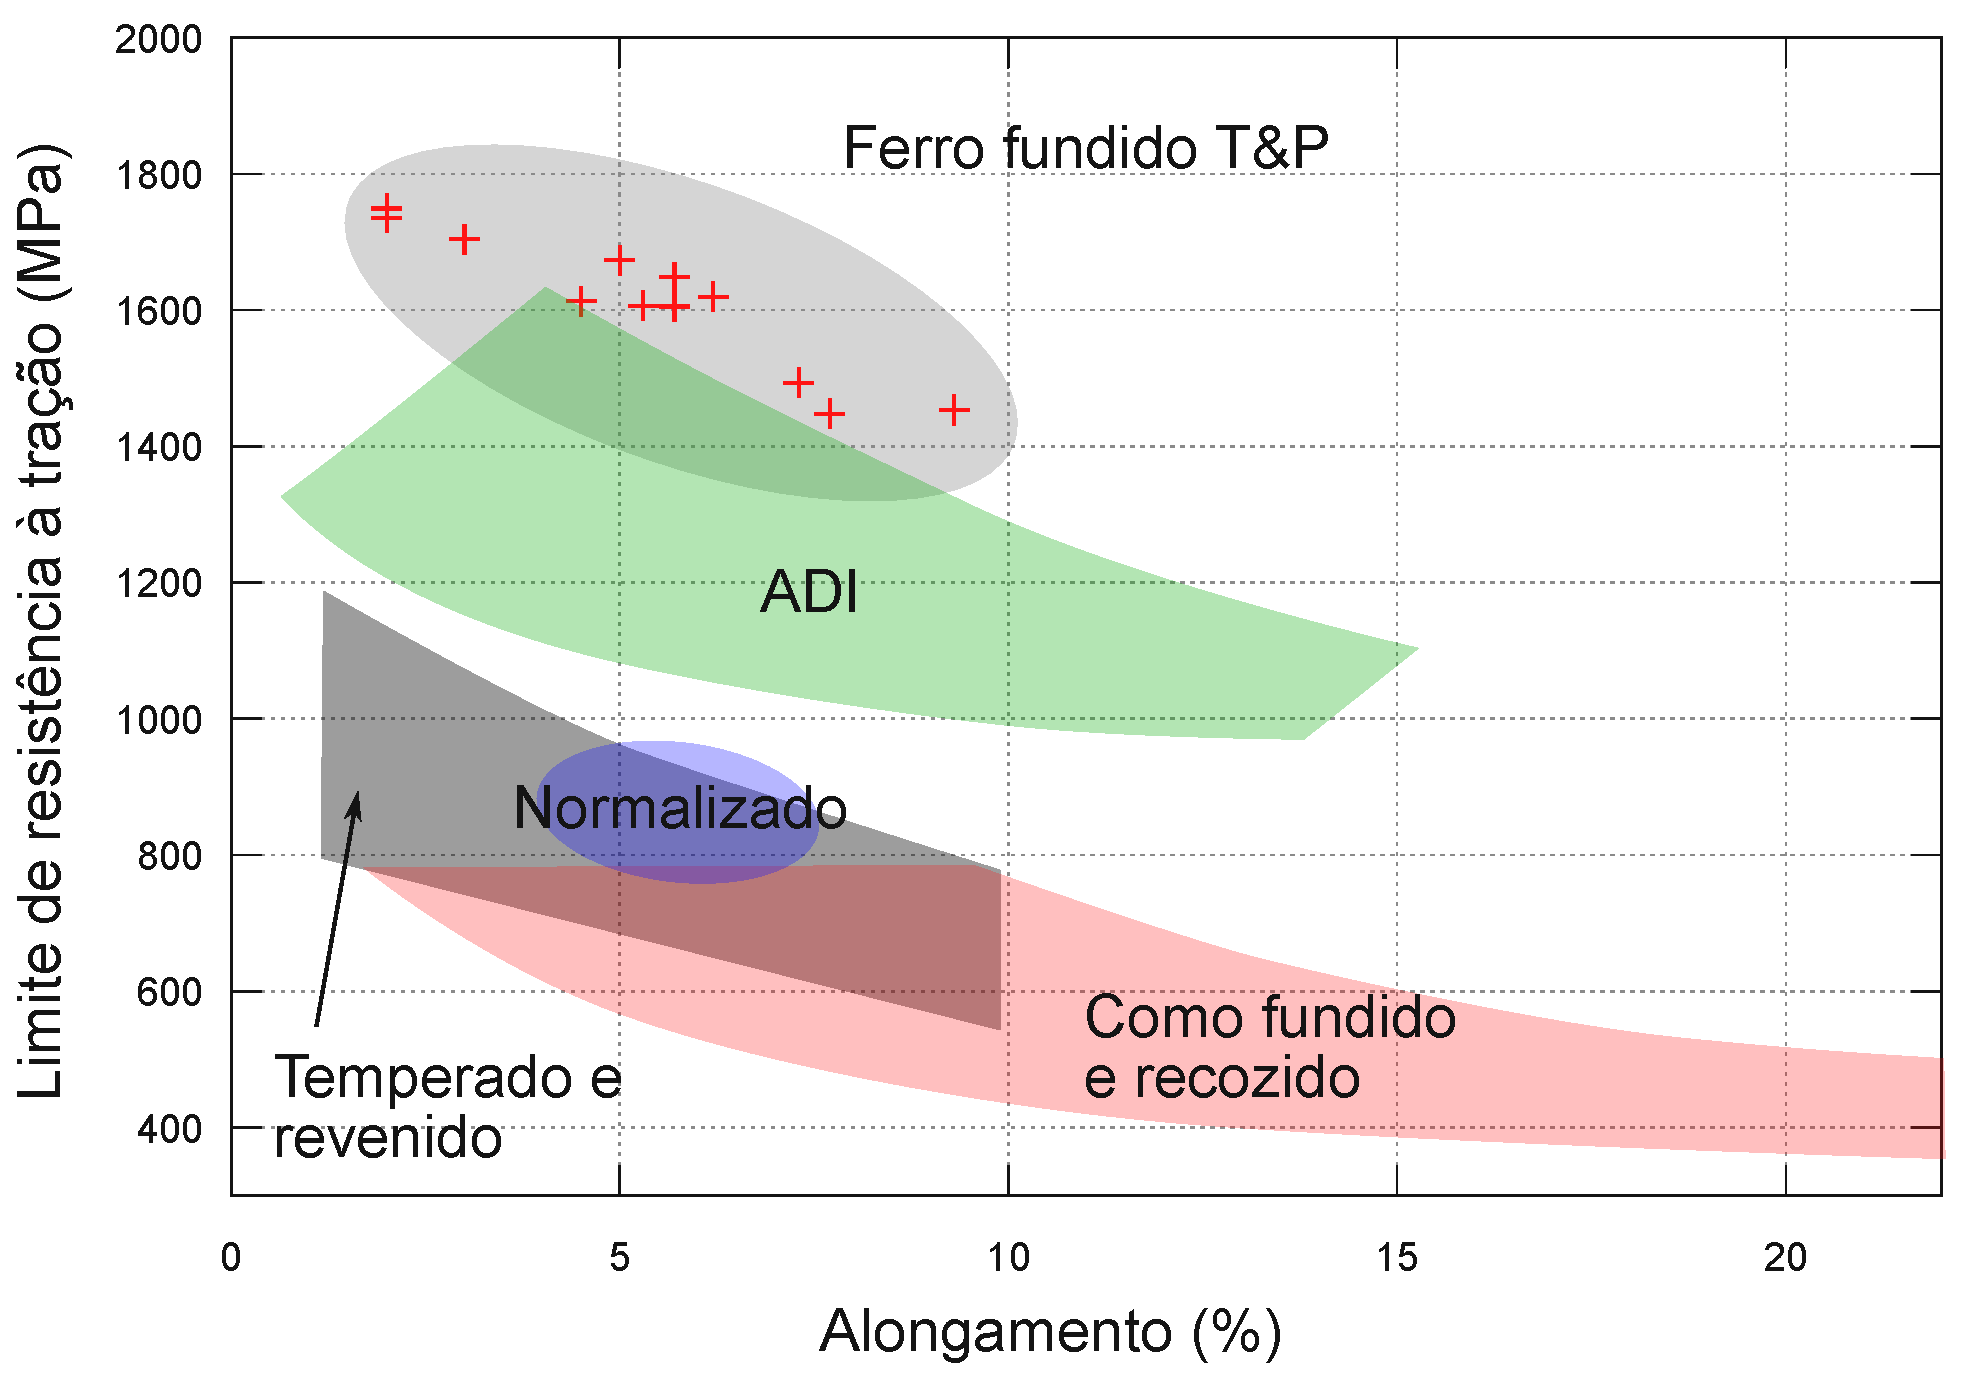
\includegraphics[width=\textwidth]{img/banana_plot-pt.pdf}
  \caption{Comparação das propriedades mecânicas do ferro fundido T\&P com diferentes classes de ferros fundidos nodulares. Adaptado de \cite{Melado2018}}
  \label{fig:banana_plot}
\end{figure}